\section{Polarizace}
\label{chap:polarizace}

Pro popis světla ve volném prostoru ($\varepsilon=1$) se dále omezíme na reálné $\vec{N}$.
Zvolíme osu $z$ proti směru šíření, tedy $\vec{N}=(0,0,-1)^T$.
Řešením jsou pole charakterizovaná libovolnými komplexními amplitudami $E_x$ a $E_y$, které udávají polarizaci vlny.
$\vec{H}$ je pak dáno rovnicí \eqref{eqn:rot-E}.

Výkon přenášený rovinou vlnou je dán časově středovaným Poyntingovým vektorem $\vec{S}$, pro vakuum\cite{bornPrinciplesOpticsElectromagnetic1999}
\begin{equation} \label{eqn:Poynting}
    \langle \vec{S}(t)\rangle_t=\langle\vec{E}(t)\times\vec{H}(t)\rangle_t=\frac{1}{2 Z_0}\vec{N} \left( E_x^*E_x+E_y^*E_y \right)
    \equiv \frac{1}{2 Z_0}\vec{N} I\,,
\end{equation}
kde definujeme normovanou intenzitu $I=E_{0x}^*E_{0x}+E_{0y}^*E_{0y}$.

Vektor $\vec{E}$ opisuje v čase obecně elipsu v rovině kolmé na směr šíření, popisné parametry definujeme podle obr. \ref{fig:polarizacni-elipsa}.
Jedná se o $\beta$ -- úhel natočení hlavní poloosy polarizace, a $\chi$ -- úhel elipticity, zde dále nazývaný zkráceně elipticita.
Pro popis ekvivalentní $E_x$ a $E_y$ je třeba přidat intenzitu $I$ a časový posun $\delta$, který má význam času, ve kterém $\vec{E}(t)$ protíná hlavní poloosu s

Konvenci točivosti světla používáme následující: při podle pohledu \emph{od zdroje} obíhá pravotočivé světlo v dané rovině po směru hodinových ručiček.
Točivost se v parametrech projevuje vzájemným znaménkem $\chi$ a točivosti systému, ve kterém je $\chi$ definováno (viz další oddíl).
Viz obr. \ref{fig:polarizacni-elipsa}.

\begin{figure}[htbp]
    \centering
    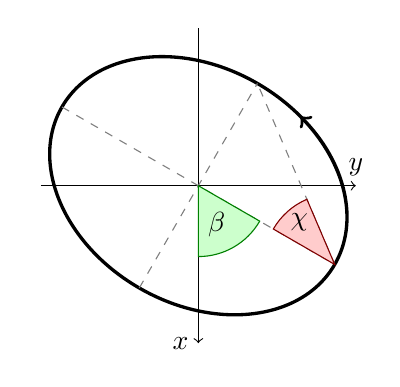
\begin{tikzpicture}[osy/.style={color=gray,dashed}]
    \draw[->] (-2,0) -- (2,0) node[anchor=south] {$y$};
    \draw[->] (0,2) -- (0,-2) node[anchor=east] {$x$};
    \draw[rotate=330,->,very thick] (2,0) arc [start angle=0, end angle=430, x radius=2cm, y radius=1.5cm];

    \draw[osy] (-30:-2cm) -- (-30:2cm);
    \draw[osy] (60:-1.5cm) -- (60:1.5cm);

    \draw[osy] (-30:2cm) -- (60:1.5cm);

    \filldraw[fill=green!20,draw=green!50!black] (0,0) -- (0,-0.9cm) arc[start angle=270, end angle=330, radius=0.9cm] -- cycle;
    \path (295:0.55cm) node {$\beta$};

    \filldraw[fill=red!20,draw=red!50!black] (330:2cm) -- (330:1.1cm) arc[start angle=150, end angle=113.13, radius=0.9cm] -- cycle;
    \path (330:2cm) ++(130:0.7cm) node {$\chi$};


\end{tikzpicture}

    \caption{Polarizační elipsa s vyznačenou soustavou souřadnou a elipsometrickými úhly $\beta$ a $\chi$ (na obrázku jsou oba kladné).
    Pro vyznačený směr svazku $\vec{k}$ se jedná o levotočivé světlo (čtenář je v pozici pozorovatele od zdroje).}
    \label{fig:polarizacni-elipsa}
\end{figure}

\subsection{Jonesův počet}
\label{chap:Jones}

Jonesovy vektory\cite{azzamEllipsometryPolarizedLight1977} jsou tvořeny přímo komplexními amplitudami polí v rovině kolmé na vektor šíření
\begin{equation}
    \J=\begin{pmatrix} E_{x} \\ E_{y} \end{pmatrix} \,.
\end{equation}

Prostor Jonesových vektorů je přirozeně normovaný intenzitou \eqref{eqn:Poynting}, která je dána skalárním součinem
\begin{equation}
    \J_1^\dagger \J_2= \begin{pmatrix} J_{1x}^* & J_{1y}^* \end{pmatrix}
    \begin{pmatrix} J_{2x} \\ J_{2y} \end{pmatrix} \,, 
    \qquad I(\J)=\J^\dagger \J
\end{equation}
Dvě polarizace/Jonesovy vektory jsou ``ortogonální'' ($\J_1^\dagger \J_2=0$), pokud je celková intenzita prostý součet intenzit v obou polarizacích.

Akci každého lineární polarizačního prvku, lze popsat jako lineární transformaci Jonesova vektoru -- transformaci Jonesovou $2\times 2$ komplexní maticí $\mathcal{T}$.
Jonesovy matice lze použít pro popis polarizačního děliče: každé rameno pak má vlastní matici.

Sadě parametrů $\beta$, $\chi$, $I$, $\delta$ odpovídá Jonesův vektor\todo{znaminka}
\begin{equation} 
\label{eqn:Jones-elipsa}
    \J=\sqrt{I} e^{i\delta} \begin{pmatrix}
        \cos \chi \cos \beta - i \sin \chi \sin \beta \\
        \cos \chi \sin \beta + i \sin \chi \cos \beta
    \end{pmatrix} \,.
\end{equation}

Zde je na místě poznámka o točivosti.
Pozdeji budeme pro usnadnění práce s téměř kolmým odrazem používat stejné souřadnice $x,y$ i pro světlo v opačném směru; vztažná soustava pak ale bude mít opačnou točivost.
V této věci se nevyhneme nějakému kompromisu, a proto přestože točivost světla je definovaná vždy vzhledem ke směru šíření, elipsometrické parametry definujeme vždy vzhledem k dané soustavě Jonesových vektorů, která může spolu se směrem šíření tvořit jak levotočivý, tak pravotočivý systém.
$\beta$ definujeme vzhledem k $J_x$, s rostoucím úhlem ve směru $+J_y$.
$\delta/\omega$ značí čas, ve kterém $\vec{E}$ protne hlavní poloosu, a vztah mezi znaménkem $\chi$ a točivostí je dán následující poučkou: pokud $J_1 J_2 \vec{k}$ tvoří levotočivý systém jako na obr. \ref{fig:polarizacni-elipsa}, pak $\chi>0$ odpovídá levotočivé polarizaci.

Při této konvenci se kruhově polarizované světlo $\J_\textrm{i}=(1, i)^T$ při kolmém dopadu odrazí se stejným Jonesovým vektorem $\J_\textrm{r}=(1, i)^T$ (a tedy stejným znaménkem $\chi$), avšak jde o opačnou točivost.


\subsection{Stokesův-Muellerův počet}
\label{chap:Stokes-Mueller}

Ucelený přehled, ze kterého vychází tento oddíl, lze nalézt v \cite{gilReviewMuellerMatrix2014,ossikovskiPoincareSphereMapping2013}.
Stokesovy parametry obecně mohou narozdíl od Jonesových vektorů popsat i nepolarizované světlo,
v této práci si však vystačíme s plně polarizovaným světlem a proto je nebudeme definovat obecně, ale pomocí Jonesových vektorů
\begin{alignat}{3}
    s_0 &\equiv J_x^* J_x+J_y^* J_y &\equiv \J^\dagger \sigma_0 \J &= I \,,\\
    s_1 &\equiv J_x^* J_x-J_y^* J_y &\equiv \J^\dagger \sigma_1 \J &= I \cos 2\chi \cos 2\beta \,,  \\
    s_2 &\equiv J_x^* J_y+J_y^* J_x &\equiv \J^\dagger \sigma_2 \J &= I \cos 2\chi \sin 2\beta \,, \\
    s_3 &\equiv i J_x^* J_y-i J_y^* J_x  &\equiv \J^\dagger \sigma_3 \J &= I \sin 2\chi \,.
\end{alignat}
kde jsme je druhými rovnostvi vyjádřili jako střední hodnoty vhodných $2\times 2$ hermitovských matic $\sigma_{i}$. Ty jsou
\begin{align}
    \sigma_0=\begin{pmatrix} 1 & 0 \\ 0 & 1 \end{pmatrix} ,\,
    \sigma_1=\begin{pmatrix} 1 & 0 \\ 0 & -1 \end{pmatrix} ,\,
    \sigma_2=\begin{pmatrix} 0 & 1 \\ 1 & 0 \end{pmatrix} ,\,
    \sigma_3=\begin{pmatrix} 0 & i \\ -i & 0 \end{pmatrix}
\end{align}
a můžeme je rozeznat jako jednotkovou matici a přerovnané Pauliho matice.
Tvoří komplexní bázi obecných komplexních $2\times 2$ matic, s omezením na reálné koeficienty pak bázi hermitovských matic. 

Každý optický prvek lineární v Jonesových vektorech je zároveň lineární ve Stokesových parametrech
\begin{equation} 
\label{eqn:Muellerova-matice}
    s^\textrm{out}_i=\J^\dagger \mathcal{T}^\dagger \sigma_i \mathcal{T} \J\equiv\J^\dagger \left(\sum_{j=0}^{3} M_{ij} \sigma_j \right) \J
    =\sum_{j=0}^{3} M_{ij} s^\textrm{in}_j \,,
\end{equation}
kde reálná $4\times 4$ matice $\M$ je dána právě rozkladem hermitovských matic $\mathcal{T}^\dagger \sigma_i \mathcal{T}$ do báze $\sigma_j$.
Matice $\M$ charakterizující optický prvek se nazývá Muellerova matice, a sloupcový vektor $\Stks$ složený ze Stokesových parametrů se nazývá Stokesův vektor.
Složky Muellerovy matice příslušející Jonesově matici $\mathcal{T}$ je možné počítat přímo z rozkladu \eqref{eqn:Muellerova-matice} díky tzv. trace-ortogonalitě $\sigma_j$ matic: $\operatorname{Tr}\lbrace\sigma_j\sigma_i\rbrace=2\delta_{ji}$
\begin{equation} 
\label{eqn:Mueller-rozklad}
    M_{ij}=\frac{1}{2}\operatorname{Tr}\lbrace \sigma_j \mathcal{T}^\dagger \sigma_i \mathcal{T} \rbrace \,.
\end{equation}

Pro plně polarizované světlo nejsou Stokesovy parametry nezávislé, platí totiž
\begin{equation} 
\label{e:norma S}
    s_0=\sqrt{s_1^2+s_2^2+s_3^2}
\end{equation}
a tedy k vyjádření polarizačního stavu stačí \emph{redukovaný} Stokesův vektor $(s_1, s_2, s_3)^T$, který lze graficky zanést do třírozměrného prostoru.
Polarizace s jednotkovou intenzitou se zobrazují na tzv. Poincarého sféře jako na obr. \ref{fig:Poincareho-sfera}.
Ortogonální polarizace jsou zobrazeny na body středově souměrné podle počátku.

\begin{figure}[htbp]
    \centering
    \input{./img/asy/poincareho-sfera.asy}
    \caption{Poincarého sféra. Je vyznačen rovník lineárních polarizací (rovina $s_3=0$, $\chi=0$) a póly kruhových polarizací $\chi=\pm 1$.}
    \label{fig:Poincareho-sfera}
\end{figure}

I Muellerovy matice musí splňovat určité podmínky.
Přestože libovolná myslitelná 4x4 reálná matice je dána 16 reálnými parametry, nedepolarizační (také nazývaná čistá\footnote{Ve smyslu čistého (nesmíšeného, angl. pure) stavu v kvantové mechanice.}) Muellerova matice je dána pouze 7 reálnými čisly\footnote{Jonesova matice je dána 4 komplexními čísly --- 8 reálných parametrů, ale při přechodu k Muellerově matici ztratíme informaci o celkové fázi.}. \cite{ossikovskiDifferentialMatrixFormalism2011}

Dále se zaměříme na to, jakým způsobem působí čisté Muellerovy matice, a jak jejich akci znázornit \emph{zobrazením Poincarého sféry}\cite{gilReviewMuellerMatrix2014,ossikovskiPoincareSphereMapping2013}.
V případě depolarizačních prvků se ke znázornění používá trojice tzv. charakteristických elipsoidů, pro čisté prvky stačí zkoumat, jakým způsobem se změní body ležící na Poincarého sféře.

Nejdříve spomeneme větu z lineární algebry o polárním rozkladu matice\cite{motlPestujemeLinearniAlgebru2002}: Každou komplexní matici $\mathcal{T}$ lze jednoznačně rozložit na součin unitární $\mathcal{U}$ a pozitivně semidefinitní hermitovské $\mathcal{H}_1, \mathcal{H}_2$ matice v libovolném pořadí, $\mathcal{T}=\mathcal{U}\mathcal{H}_1 = \mathcal{H}_2 \mathcal{U}$.

\paragraph{Čistý retardér}

Prvek reprezentovaný unitární Jonesovou maticí $\mathcal{U}$ zachovává intenzitu a projevuje se pouze fázovým zpožděním mezi dvěma ortogonálními polarizacemi.
Zachovává intenzitu, takže Poincarého sféra nebude deformovaná ani posunutá, pouze otočená či převrácená.
$\mathcal{U}$ lze diagonalizovat a její vlastní čísla jsou komplexní fázové faktory, píšeme tedy\footnote{Ve vzorci vystupuje dyadický součin Jonesových vektorů $\J\J^\dagger$, což je ortogonální projektor na $\J$, ne skalární součin, který by byl psaný $\J^\dagger \J$.}
\begin{equation}
    \mathcal{U}=e^{i\Delta_1} \J_1 \J_1^\dagger + e^{i\Delta_2} \J_2 \J_2^\dagger\,.
\end{equation}
Tyto dva vlastní módy mají po průchodu prvkem stejný polarizační stav, akce Muellerovy matice na Poincarého sféru má tedy za následek rotaci sféry kolem osy procházející těmito vlastními módy.
Úhel rotace je dán fázovým zpožděním $\Delta=\Delta_1-\Delta_2$.
Ve speciálním případě $\J_1=(1,0)^T$ a $\J_2=(0,1)^T$ je Jonesova a Muellerova matice\todo{zkontrolovat znaminka toho uhlu}
\begin{equation}
\label{eqn:cisty-retarder}
    \mathcal{U}=\begin{pmatrix}
        e^{i\Delta_1} & 0 \\ 0 & e^{i\Delta_2}
        \end{pmatrix} \,, \qquad
    \mathbb{U}=\begin{pmatrix}
        1 & 0 & 0 & 0 \\ 0 & \cos\Delta & \sin\Delta & 0 \\
        0 & -\sin\Delta & \cos\Delta & 0 \\ 0 & 0 & 0 & 1
        \end{pmatrix} \,.
\end{equation}

\paragraph{Čistý diatenuátor}

Pro prvek reprezentovaný pozitivně semidefinitní hermitovskou Jonesovou maticí $\mathcal{H}$ existují dva ortogonální vlastní módy s reálnými nezápornými vlastními čísly -- různými koeficienty útlumu.
Normalizací matice tak, že větší z vlastních čísel se rovná 1, lze psát s reálným nezáporným $\eta$
\begin{equation}
    \mathcal{H}=\J_1 \J_1^\dagger + \eta \J_2 \J_2^\dagger \,.
\end{equation}

Jedná se o obecný polarizátor, který $\J_1$ propustí zcela a $\J_2$ propustí s amplitudovou propustností $\eta$.
Ve speciálním případě $\J_1=(1,0)^T$ a $\J_2=(0,1)^T$ je Jonesova a Muellerova matice
\begin{equation}
    \mathcal{H}=\begin{pmatrix}
        1 & 0 \\ 0 & \eta
        \end{pmatrix} \,, \qquad
    \mathbb{H}=\begin{pmatrix}
        \frac{1+\eta^2}{2} & \frac{1-\eta^2}{2} & 0 & 0 \\ \frac{1-\eta^2}{2} & \frac{1+\eta^2}{2} & 0 & 0 \\
        0 & 0 & \eta & 0 \\ 0 & 0 & 0 & \eta
        \end{pmatrix} \,.
\end{equation}

Pro body na Poincarého sféře dosadíme $s_0^\textrm{in}=1$ a dostaneme
\begin{equation}
    \begin{pmatrix} s_1 \\ s_2 \\ s_3 \end{pmatrix}_{\textrm{out}}
    =\begin{pmatrix} \frac{1+\eta^2}{2} & 0 & 0 \\ 0 & \eta & 0 \\ 0 & 0 & \eta \end{pmatrix}
    \begin{pmatrix} s_1 \\ s_2 \\ s_3  \end{pmatrix}_{\textrm{in}}
    +\begin{pmatrix} \frac{1-\eta^2}{2} \\ 0 \\ 0 \end{pmatrix}
\end{equation}
Jedná se tedy o kontrakci v rovině $s_2s_3$ faktorem $\eta$, ve směru $s_1$ faktorem $(1+\eta^2)/2$ a zároveň posunutím o $(1-\eta^2)/2$.
Ekvivalentně lze mluvit o kontrakcí stejným faktorem se středem\footnote{$(s_1^\textrm{out}-1)=(s_1^\textrm{in}-1)(1-\eta^2)/2$.} v $s_3=1$.
Se zmenšujícím $\eta$ (vyšší kvalitou polarizátoru) výsledný elipsoid svým tvarem nabývá podobnosti doutníku.

Shrneme-li uvedené poznatky, akce libovolného nedepolarizačního optického prvku je ekvivalentní postupnému působení obecného diatenuátoru (protáhnutí a posunutí ve směru vlastního vektoru $\mathcal{H}$ jako na obr. \ref{fig:UH-Mueller} (b)) a obecného retardéru (rotace podle směru vlastního vektoru $\mathcal{U}$ jako na obr. \ref{fig:UH-Mueller} (a)), případně v opačném pořadí.

Zobrazení Poincarého sféry nachází využití především pro depolarizační Muellerovy matice, ale i v našem případě nabízí jednoduchý intuitivní způsob přemýšlení o polarizaci, který je důležitý např. při rychlých rozhodnutích v laboratoři, kdy není čas násobit komplexní matice.

\begin{figure}[htbp]
    \centering
    \begin{subfigure}{.3\textwidth}
        \centering
        \input{./img/asy/akce-muelleru-U.asy}
    \end{subfigure}
    \begin{subfigure}{.67\textwidth}
        \centering
        \input{./img/asy/akce-muelleru-H.asy}
    \end{subfigure}
    \caption{Zobrazení Poincarého sféry čistými Muellerovými maticemi. (a) čistý retardér (rotace sféry), (b) čistý diatenuátor (protáhnutí a posunutí sféry).}
    \label{fig:UH-Mueller}
\end{figure}
